\documentclass[12pt]{article}

\usepackage[utf8]{inputenc}
\usepackage[T1]{fontenc}
\usepackage{datetime}
\usepackage[spanish]{babel}
\usepackage{graphicx}
\usepackage{listings}
\usepackage{caption}
\usepackage{subcaption}
\usepackage[right=2cm,left=2cm,top=2cm,bottom=2cm]{geometry}
\usepackage{hyperref}
\usepackage{fancyhdr}
\usepackage{color}
\usepackage[export]{adjustbox}
\usepackage{graphicx}
\usepackage{float}
\usepackage{changepage}
\usepackage{multicol}
\usepackage{imakeidx}
\usepackage{csquotes}
\usepackage{array}
\usepackage{tabularx}
\usepackage{xcolor}
\usepackage[backend=biber]{biblatex}
\addbibresource{webgrafia.bib}

\pagestyle{fancy}
\renewcommand{\footrulewidth}{0.4pt}
\setlength{\headheight}{15pt}


\fancyhead[L]{ CEIABD – SBD }
\fancyhead[R]{ Páez Anguita, Víctor }
\fancyfoot[L]{IES Gran Capitán}


\begin{document}

\begin{titlepage}
    \begin{center}
      \Large \bfseries{}
    \end{center}
    \vspace{0.1cm}
    \begin{center}
      \Large \bfseries{}
    \end{center}
    \vspace{0.1cm}
    \begin{center}
     \Large \bfseries{Estructuración de datos}
    \end{center}
    \vspace{0.0001cm}
    \begin{center}
        Departamento de informática \\ I.E.S. Gran Capitán - Córdoba
    \end{center}
        \vspace{2 cm}
\begin{figure}[h!]
    \centering
    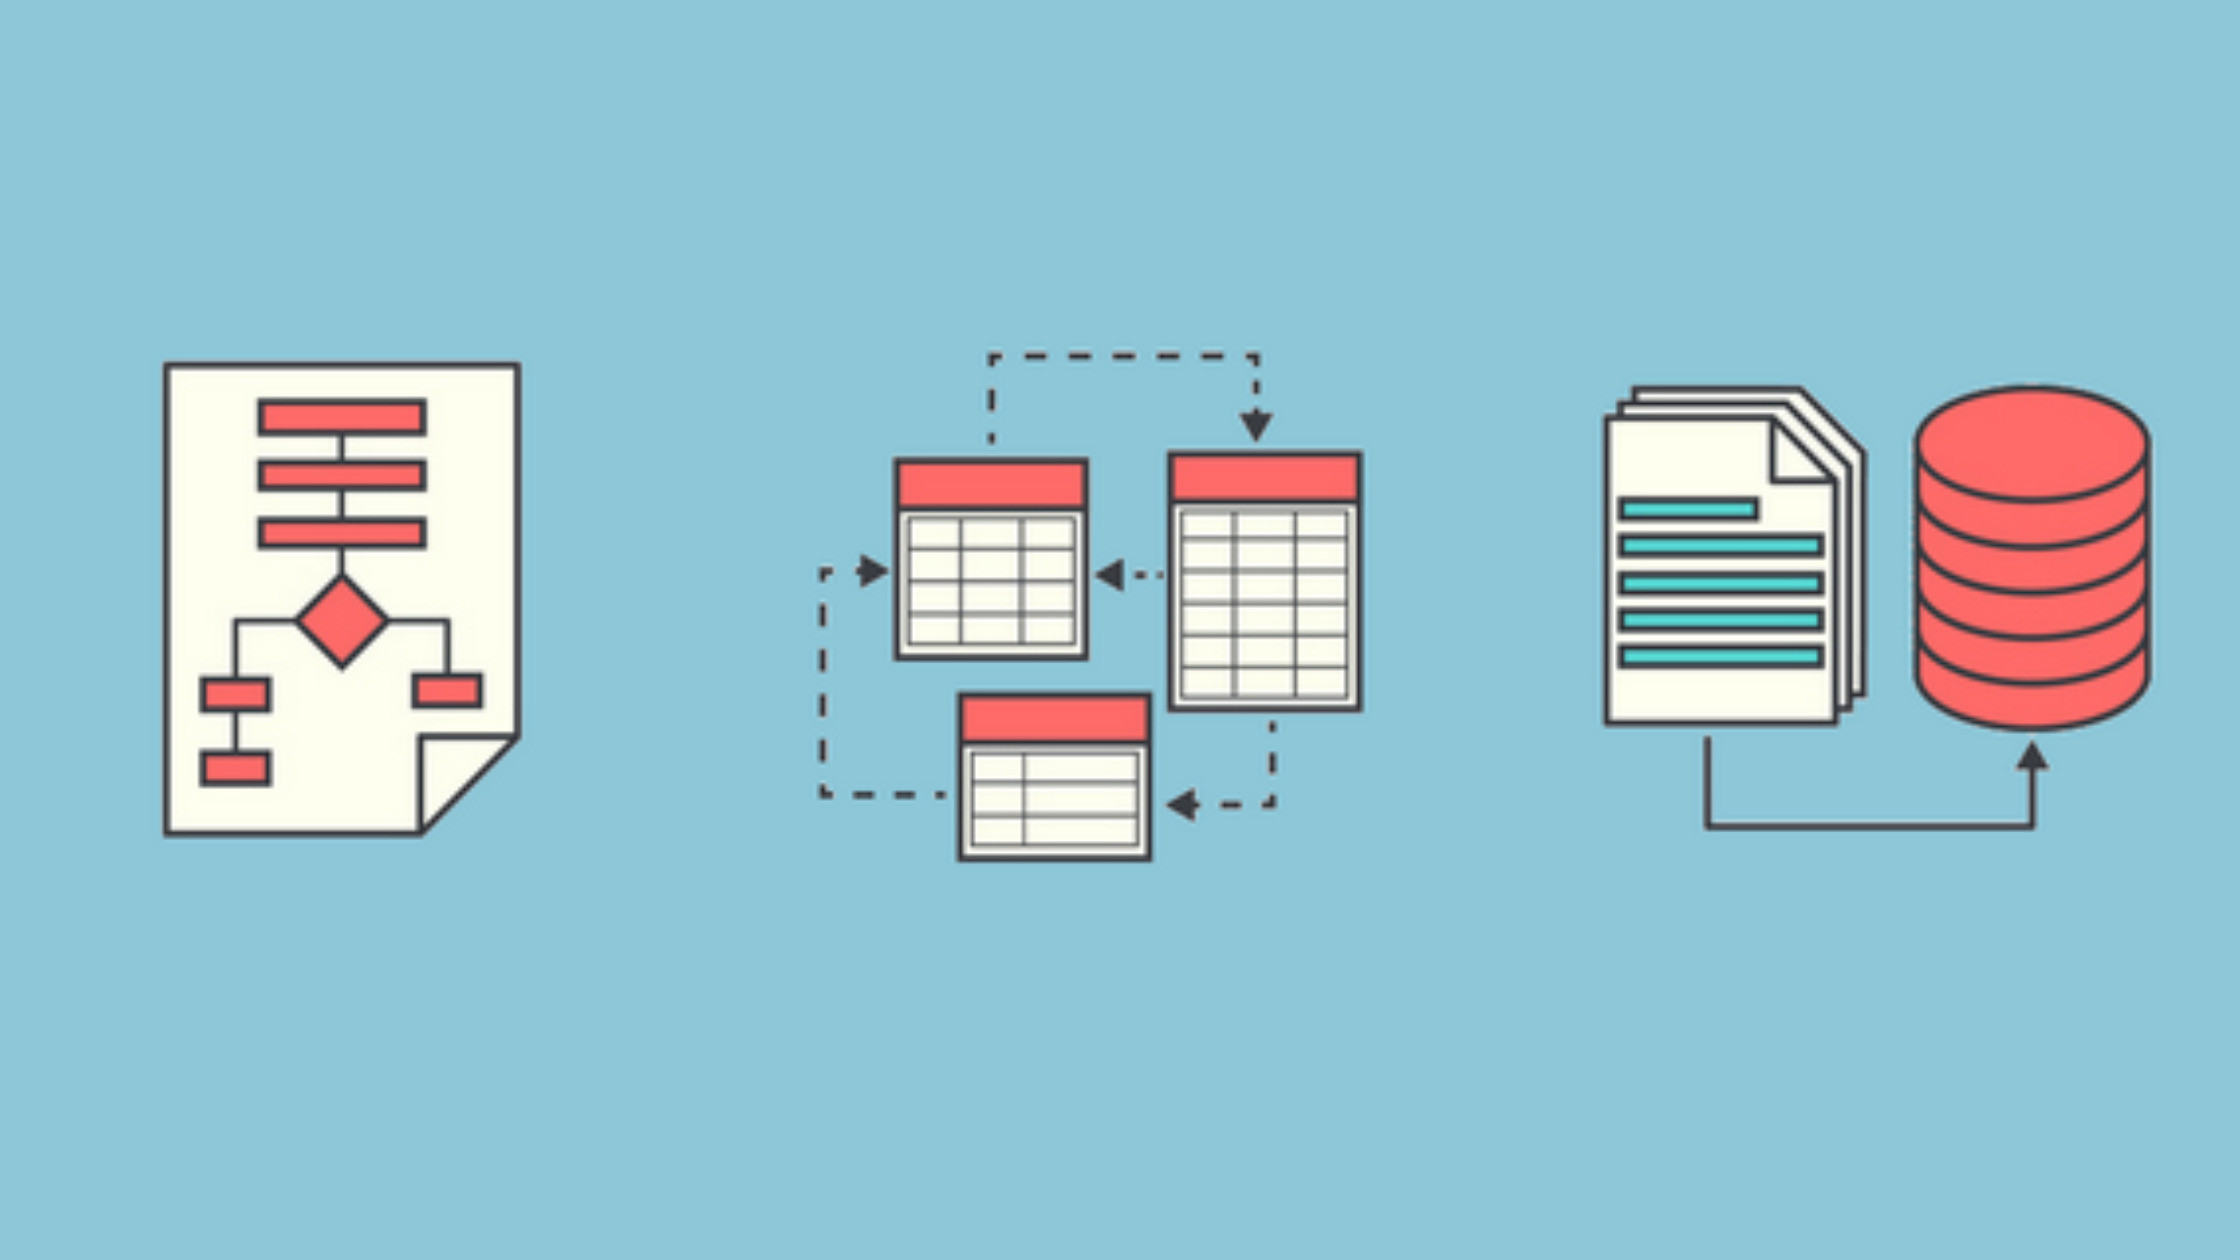
\includegraphics[width=.6\textwidth]{portada.jpg}
    \label{fig:my_label}
\end{figure}
    \vspace{0.2 cm}
    \begin{center}
        Inteligencia artificial y Big data \\ \today 
    \end{center}
    \vspace{4 cm}
\null\hfill \textbf{Desarrollado por:}
\\
\\
\null\hfill Víctor Páez Anguita
\clearpage
\end{titlepage}

%%%%%%%%%%%%%%%%%%%%%%%%%%%Index%%%%%%%%%%%%%%%%%%%%%%%%%%%%%%%%
\tableofcontents
\clearpage
%%%%%%%%%%%%%%%%%%%%%%%%%%%Index%%%%%%%%%%%%%%%%%%%%%%%%%%%%%%%%


\section{Ejemplo de la vida real de la transformación de datos en conocimiento}

\textbf{Medicina personalizada y predicción de enfermedades}

\begin{itemize}
    \item \textbf{Datos}
    \\
    Los datos en medicina provienen de diversas fuentes, como:
    \begin{itemize}
        \item Historiales médicos
        \item Resultados de pruebas de laboratorio
        \item Imágenes médicas
        \item Datos genéticos
        \item Datos de sensores
    \end{itemize}

    \item \textbf{Información}
    Una vez recopilados los datos, se organizan en bases de datos médicas y se procesan con herramientas de inteligencia artificial 
    y análisis estadístico. Algunos ejemplos de información generada son:
    \begin{itemize}
        \item Patrones en la salud del paciente:
            \begin{itemize}
                \item Se observa que una persona con ciertos genes tiene un 60\% más de riesgo de desarrollar diabetes tipo 2.
                \item Un paciente con presión alta y alto colesterol tiene una mayor probabilidad de sufrir un infarto en los próximos 10 años.
            \end{itemize}
        \item Clasificación de pacientes:
            \begin{itemize}
                \item Pacientes con riesgo bajo, medio o alto de desarrollar enfermedades cardiovasculares.
                \item Agrupaciones de pacientes según respuesta a ciertos medicamentos.
            \end{itemize}
    \end{itemize}

    \item \textbf{Conocimiento}
    \\
    Con la información obtenida, los médicos pueden tomar decisiones personalizadas y basadas en evidencia:
    \begin{itemize}
        \item Prevención y cambios en el estilo de vida
            \begin{itemize}
                \item Si un paciente tiene alta probabilidad de desarrollar diabetes, el médico recomienda cambios en la dieta y 
                actividad física antes de que la enfermedad aparezca.
                \item Se pueden diseñar programas personalizados de prevención para cada paciente según sus factores de riesgo.
            \end{itemize}
        \item Tratamientos personalizados
            \begin{itemize}
                \item Se determina que ciertos pacientes metabolizan mejor un medicamento específico, evitando efectos 
                secundarios graves.
                \item Se ajusta la dosis de fármacos en función del perfil genético del paciente.
            \end{itemize}
        \item Predicción de enfermedades
            \begin{itemize}
                \item Algoritmos de IA analizan datos médicos de miles de pacientes para detectar patrones que indiquen 
                la aparición temprana de enfermedades como cáncer o Alzheimer.
                \item Se pueden hacer alertas tempranas para que el médico realice chequeos más frecuentes en pacientes con 
                alto riesgo.
            \end{itemize}
    \end{itemize}
\end{itemize}

\clearpage
\section{Diferencias entre un data lake y un data warehouse}

\renewcommand{\arraystretch}{2} % Espaciado vertical en las celdas

\begin{table}[h]
    \centering
    \begin{tabular}{|p{3.5cm}|p{6cm}|p{5.8cm}|}
        \hline
        \textbf{Característica} & \textbf{Data Lake} & \textbf{Data Warehouse} \\
        \hline
        \textbf{Tipos de datos} & Datos estructurados, semiestructurados y no estructurados (logs, imágenes, videos, texto, etc.) & Principalmente datos estructurados y algunos semiestructurados \\
        \hline
        \textbf{Objetivo} & Almacenar grandes volúmenes de datos en su forma original para análisis posterior & Proporcionar información estructurada y optimizada para análisis y generación de reportes \\
        \hline
        \textbf{Flexibilidad} & Alta, permite almacenar cualquier tipo de datos sin necesidad de una estructura definida & Baja, requiere modelado previo y esquemas estructurados \\
        \hline
        \textbf{Procesamiento} & ETL (Extract, Load, Transform) o ELT (Extract, Load, Transform) según el uso & ETL (Extract, Transform, Load), donde los datos se transforman antes de almacenarse \\
        \hline
        \textbf{Velocidad de acceso} & Baja, requiere procesamiento adicional para consultas & Alta, optimizado para consultas rápidas y reportes \\
        \hline
        \textbf{Costo} & Menor, usa almacenamiento escalable y económico (ej. HDFS, S3) & Mayor, requiere procesamiento optimizado y almacenamiento estructurado \\
        \hline
        \textbf{Casos de uso} & Machine Learning, Big Data Analytics, almacenamiento de datos históricos sin procesar & Business Intelligence, reportes financieros, análisis de tendencias empresariales \\
        \hline
        \textbf{Usuarios principales} & Científicos de datos, ingenieros de datos, analistas avanzados & Analistas de negocio, ejecutivos, gerentes de TI \\
        \hline
        \textbf{Herramientas comunes} & Hadoop, Apache Spark, Amazon S3, Google Cloud Storage, Azure Data Lake & Amazon Redshift, Google BigQuery, Snowflake, Teradata, Microsoft SQL Server \\
        \hline
    \end{tabular}
    \label{tab:data_lake_vs_warehouse}
\end{table}


\clearpage

\section{ejemplo real de los 4 tipos de analítica}

Como ejemplo voy a usar una plataforma de streaming de video como Netflix que analiza
el comportamiento de sus usuarios para mejorar la recomendación de contenido y optimizar su plataforma.

\subsection{descriptiva}

La analítica descriptiva resume y organiza datos históricos para comprender qué ha ocurrido en la plataforma.
\\
Ejemplo:

\begin{itemize}
    \item El equipo de análisis observa que el 70\% de los usuarios ven series de drama después de las 8 p.m.
    \item Se detecta que las películas de ciencia ficción tienen una tasa de finalización del 80\%,
    mientras que los documentales solo el 40\%.
\end{itemize}

Herramientas usadas: Dashboards, reportes, estadísticas básicas.

\subsection{diagnóstica}

Aquí se analizan las causas detrás de los patrones detectados en la analítica descriptiva.
\\
Ejemplo:
\begin{itemize}
    \item Al analizar los datos de visualización, se descubre que los usuarios ven más series de drama en
    la noche porque suelen relajarse después del trabajo.
    \item Se encuentra que los documentales tienen una menor tasa de finalización porque suelen ser más largos y 
    con menos cliffhangers que otras categorías.
\end{itemize}

Herramientas usadas: Análisis de correlación, segmentación de clientes, minería de datos.

\subsection{predictiva}

La analítica predictiva usa modelos de machine learning y estadísticas avanzadas para anticipar futuros comportamientos.
\\
Ejemplo:

\begin{itemize}
    \item Basándose en el historial de visualización, el sistema predice que los usuarios que ven thrillers psicológicos 
    también disfrutarán de series de misterio.
    \item Se proyecta que si una nueva temporada de una serie popular se lanza un viernes por la noche, 
    las visualizaciones aumentarán en un 40\% durante el fin de semana.
\end{itemize}

\subsection{prescriptiva}

Aquí se generan recomendaciones y estrategias basadas en los resultados de la analítica predictiva.
\\
Ejemplo:
\begin{itemize}
    \item La plataforma decide promocionar contenido de misterio a los usuarios que ven thrillers psicológicos, 
    aumentando la retención de espectadores.
    \item Se recomienda lanzar nuevas temporadas los viernes por la noche para maximizar la audiencia.
    \item Se ajusta el algoritmo de recomendaciones para dar prioridad a los contenidos con alta tasa de finalización, 
    asegurando que los usuarios se enganchen con el contenido sugerido.
\end{itemize}

Herramientas usadas: Sistemas de recomendación, optimización, simulaciones.

\section{Ejemplo real de catastrofe por culpa del big data con el bussines intelligence}

\textbf{La Crisis de Target y la Privacidad de los Clientes}

Uno de los casos más controversiales en el uso de Big Data ocurrió con Target, la cadena de supermercados en EE.UU., 
cuando su sistema de análisis predictivo provocó una crisis de privacidad en 2012.

\textbf{¿Qué ocurrió?}

Target implementó un sistema de Big Data y analítica predictiva para identificar patrones de compra de sus clientes y 
predecir futuras necesidades. En este proceso, su algoritmo descubrió que ciertas combinaciones de compras 
(lociones sin fragancia, suplementos de calcio, toallas de algodón, entre otros) indicaban que una clienta probablemente 
estaba embarazada.
Utilizando estos datos, la empresa comenzó a enviar cupones y ofertas personalizadas a clientes que el sistema identificó 
como embarazadas.

\textbf{El Problema}

En un caso particular, una adolescente recibió en su casa un folleto con descuentos en productos para embarazadas, 
lo que alertó a su familia. Su padre, molesto, fue a reclamar a Target, acusándolos de fomentar el embarazo en adolescentes.

Semanas después, el padre descubrió que su hija efectivamente estaba embarazada y que Target lo había sabido antes que él, 
gracias a su análisis de datos.

\textbf{Consecuencias}

\begin{itemize}
    \item La historia se viralizó y Target fue duramente criticado por invadir la privacidad de los clientes.
    \item Se generó un debate sobre los límites éticos del Big Data y el uso de datos sin consentimiento explícito.
    \item Para evitar problemas similares, Target modificó sus estrategias de marketing, mezclando anuncios de productos 
    para embarazadas con otros no relacionados, para hacer que las predicciones fueran menos evidentes.
\end{itemize}

\section{Relación entre el big data y el bussines intelligence}

El Big Data y el Business Intelligence están estrechamente relacionados y se complementan entre sí. 
El Big Data proporciona la materia prima: los datos. El Business Intelligence, por otro lado, se encarga de procesar, 
analizar y transformar esos datos en información útil.
\\
El Big Data permite a las organizaciones acceder a grandes cantidades de datos de diferentes fuentes, 
lo que amplía su capacidad para analizar y comprender mejor su negocio y su entorno. El Business Intelligence, 
por su parte, utiliza técnicas avanzadas para extraer información valiosa de esos datos y proporcionar una visión clara 
y precisa del desempeño empresarial.

Un ejemplo podria ser:

\begin{itemize}
    \item Big Data recopila y procesa datos en tiempo real, como comentarios en redes sociales, 
    sensores IoT o registros de transacciones.
    \item BI toma esos datos procesados y los convierte en reportes comprensibles para los ejecutivos y tomadores de decisiones.
\end{itemize}

\section{Ofertas de trabajo para data science y sus requisitos}

\begin{enumerate}
    \item \href{https://www.linkedin.com/jobs/view/4160806767}{Data Scientist(Junior) TENDAM}

    What we are looking for:

    Scientific background with computational and analytical skills

    Strong problem-solving skills

    Programming skills with Python and SQL

    Understanding and experience with big data systems, especially with Spark (PySpark)

    Knowledge of a variety of machine learning techniques (clustering, regression, decision trees, neural networks, etc.)

    Experience with data visualization tools and packages

    A drive to learn and master new technologies and techniques

    Excellent written and verbal communication skills

    ~1 year of industry experience

    Extra qualifications

    Experience working with huge amounts of data

    Experience with cloud based web services (e.g., AWS)

    Knowledge and experience with a version control system (e.g. Git).

    \item \href{https://www.linkedin.com/jobs/view/4150478232}{Analista de datos(Córdoba) Grupo de Prado}
    
    Grado en: ADE, Ingeniería, Estadística, Matemáticas o Económicas.

    Power BI 
    
    Python y Knime 
    
    Bases de datos
    
    Técnicas estadísticas de análisis de datos 
    
    ArcGis (deseable)
    
    Conocimiento de negocio agrícola/ERP agrícola (deseable)
    
    Inglés C1 (deseable)

    \item \href{https://www.linkedin.com/jobs/view/4146379722}{Analista de datos Avalora}

    Análisis de datos y realización de Dashboard de KPIs, Principalmente en Power BI y valorable otras como Salesforce.

    Elaboración de informes, análisis y preparación de datos para reporting, análisis y seguimiento de datos pipeline y comparativos. 
    
    Utilización y soporte de las herramientas corporativas para la gestión comercial y registro de la actividad comercial. 
\end{enumerate}

\textbf{Que se necesita para ser un data scientist}

\begin{itemize}
    \item Conocimientos de programación: Python, R, SQL, Java, Scala, etc.
    \item Conocimientos de estadística y matemáticas: álgebra, cálculo, probabilidad, etc.
    \item Conocimientos de machine learning y data mining: algoritmos, técnicas, modelos, etc.
    \item Conocimientos de big data: Hadoop, Spark, NoSQL, etc.
    \item Conocimientos de visualización de datos: Tableau, Power BI, D3.js, etc.
    \item Conocimientos de bases de datos: MySQL, PostgreSQL, MongoDB, etc.
    \item Conocimientos de cloud computing: AWS, Azure, Google Cloud, etc.
\end{itemize}


\section{3 busquedas en google con operadores que no conocias}

\begin{itemize}
    \item Buscar resultados que contengan al menos una de varias palabras clave

    \textbf{energía solar OR energía eólica} Esta búsqueda mostrará resultados que contengan "energía solar" o "energía eólica".

    \item Buscar resultados que contengan una palabra clave en el título y otra en la URL

    \textbf{intitle:"cambio climático" inurl:informes} Esto mostrará páginas cuyo título incluya "cambio climático" y cuya URL contenga "informes".
    
    \item Buscar resultados que excluyan una palabra clave específica
    
    \textbf{recetas de pastel -chocolate} Esta búsqueda mostrará recetas de pastel que no incluyan "chocolate".
\end{itemize}

\section{Analisis de sentimiento}

Para este apartado voy a utilizar Nelsenso.Net \href{https://www.nelsenso.net/es/tonetizer.aspx}{Nelsenso.Net}.

\subsection{Restaurante}

\textbf{Restaurante el olivo}

\begin{figure}[h!]
    \centering
    \includegraphics[width=.6\textwidth]{reseña2.PNG}
    \label{fig:my_label}
\end{figure}

\begin{figure}[h!]
    \centering
    \includegraphics[width=.6\textwidth]{reseña2-2.PNG}
    \label{fig:my_label}
\end{figure}

La herramienta ha hecho un buen trabajo detectando que el comentario es positivo.

\clearpage

\subsection{Monumento}

\textbf{La Mezquita catedral de Córdoba}

\begin{figure}[h!]
    \centering
    \includegraphics[width=.6\textwidth]{reseña1.PNG}
    \label{fig:my_label}
\end{figure}

\begin{figure}[h!]
    \centering
    \includegraphics[width=.6\textwidth]{reseña1-1.PNG}
    \label{fig:my_label}
\end{figure}



En esta reseña podemos ver como el usuario ha escrito un comentario positivo sobre la mezquita, pero la herramienta 
debido ha cirtas palabras que tiene parametrizadas como mezquita o cultura ha interpretado que es un comentario negativo.

\subsection{Local}

\textbf{Pop Up Sala De Eventos}

\begin{figure}[h!]
    \centering
    \includegraphics[width=.6\textwidth]{reseña3.PNG}
    \label{fig:my_label}
\end{figure}

\clearpage

\begin{figure}[h!]
    \centering
    \includegraphics[width=.6\textwidth]{reseña3-3.PNG}
    \label{fig:my_label}
\end{figure}

La verdad que no entiendo muy bien como la herramienta ha interpretado que el comentario es negativo, ya que en el comentario
se puede apreciar muchos caracteres que son indice de un comentario positivo. Normalmente al tokenizar el texto estos 
suelen ser de los más faciles a la hora de clasificar. Supongo que la herramienta no es demasiado buena.

\clearpage

\section{Bibliografia}

\cite{Estructuracion_de_datos}
\cite{Ejemplos_reales_del_Big_Data}
\cite{Data_Lake_vs_Data_Warehouse_kaits}
\cite{Data_Lake_vs_Data_Warehouse_bismart}
\cite{Tipos_de_análisis_de_datos}
\cite{Ejemplo_real_de_catastrofe}
\cite{relacion_big_data_y_business_intelligence}
\cite{relacion_big_data_y_business_intelligence_2}
\cite{requisitos_para_ser_cientifico_de_datos}

\printbibliography

\end{document}
